% ****** Start of file apssamp.tex ******
%
%   This file is part of the APS files in the REVTeX 4.1 distribution.
%   Version 4.1r of REVTeX, August 2010
%
%   Copyright (c) 2009, 2010 The American Physical Society.
%
%   See the REVTeX 4 README file for restrictions and more information.
%
% 
\documentclass[%
aps, %aps-style journal
prl, % physical review letters
preprint, % double spaced
12pt, % 12 point font
amsfonts, % ams fonts
amssymb, % ams symbols
amsmath, % ams math  features
endfloats,% put all figures/tables at  end, one per page
raggedbottom, % allow variation at bottom
]{revtex4-1}

\providecommand{\e}[1]{\ensuremath{\times 10^{#1}}}

\usepackage{graphicx}% Include figure files
\usepackage{hyperref}

\begin{document}

\preprint{UCSB Chemistry 222B}

\title{Numerical solution to the time-independent Schrödinger equation for HCl in a Morse potential using finite difference}
% Force line breaks with \\
\author{Jackson Sheppard}
\affiliation{%
Chemistry Department, University of California, 
Santa Barbara, CA 93106-9530}

\begin{abstract}
Here we present a numerical solution to the time-independent Schrödinger equation for the diatomic molecule HCl in a Morse potential well using the method of finite difference to calculate the energy
eigenvalues and corresponding eigenstates in $r$-coordinate space, where $r$ is the interatomic
separation between the hydrogen and chlorine atoms. This method considers the continuous radial
coordinate $r$ as an evenly spaced grid of $n$ points and approximates the derivative of the
function $f(r)$ as $\Delta f/ \Delta r$. In doing so, one can solve the eigenvalue equation
$HU(r) = EU(r)$ as a discrete problem yielding $n$ energy eigenvalues $\{E_n\}$ and $n$ eigenvectors $\{U_n(r)\}$, each
evaluated at the $n$ radial coordinates. Implementing these methods for HCl using
Python yields a ground state energy $E_0 = -4.434$ eV, in excellent agreement with that found from
the analytical solution to this differential equation.
\end{abstract}

\date{February 8, 2022}
\maketitle

\section{\label{sec:Intro}Introduction}

The Morse potential $V(r)$, first introduced by Philip M. Morse, describes the interaction between
atoms in a diatomic molecule and can be thought of as the energy stored in the bond as function of atomic
separation $r$. This potential energy takes the form of an anharmonic oscillator with respect to
$r$ and thus has energy eigenvalues perturbed from that of the standard quantum harmonic
oscillator. The Morse potential takes the form:
\begin{equation} \label{morse}
    V(r) = D_e(1 - e^{-a(r - r_e)})^2 - D_e
\end{equation}
Here $D_e$ is the well-depth (the diatomic molecule dissociation energy), $r_e$ is the equilibrium
separation between the two atoms, and the parameter $a$ is defined as $a = \sqrt{k_e/2D_e}$,
where $k_e$ is the spring force constant calculated at the minimum of the well $r = r_e$.
We note that the offset of $D_e$ is arbitrary and applied for mathematical convenience. One can 
then rewrite Eq. \ref{morse} as follows:
\begin{equation} \label{morse2}
    V(r) = D_e(e^{-2a(r-r_e)} - 2e^{-a(r-r_e)})    
\end{equation}
giving the functional form employed in this analysis.

The time-independent Schrödinger equation for the wave function $U(r)$
is then:
\begin{align}
    -\frac{\hbar^2}{2m}\frac{d^2U(r)}{dr^2} + V(r)U(r) &= EU(r) \label{TISE}\\
    HU(r) &= EU(r)
\end{align}
where $m = m_Hm_{Cl}/(m_H + m_Cl)$ is the reduced mass of HCl and $H = K + V$ is the Hamiltonian operator expressed as a sum of the kinetic energy $K = (-\hbar^2/2m)d^2/dr^2$
and Morse potential energy $V = V(r)$ terms.

Next we employ the method of finite difference by approximating the derivative of the wave
function $U(r)$ evaluated at a discrete radial position $r_i$ as follows:
\begin{equation}
    \frac{dU}{dr}\Bigr|_{r=r_i} \approx \frac{\Delta U}{\Delta r}\Bigr|_{r=r_i} = \frac{U(r_{i+1}) - U(r_{i-1})}{r_{i+1} - r_{i-1}} = \frac{U_{i+1} - U_{i-1}}{2d}
\end{equation}
where $d$ is the incremental step size in $r$. To evaluate the second derivative, we consider
the Taylor expansion of the continuous function $f(x)$ shifted by small amounts $+\Delta x$ and $-\Delta x$, giving:
\begin{align}
    f(x + \Delta x) & \approx f(x) + \frac{df}{dx}\Delta x + \frac{1}{2}\frac{d^2f}{dx^2}\Delta x^2 \\
    f(x - \Delta x) & \approx f(x) - \frac{df}{dx}\Delta x + \frac{1}{2}\frac{d^2f}{dx^2}\Delta x^2
\end{align}
Adding the two expressions above yields:
\begin{align}
    f(x + \Delta x) + f(x - \Delta x) & \approx 2f(x) + \frac{d^2f}{dx^2}\Delta x^2 \\
    \frac{d^2f}{dx^2} & \approx \frac{f(x + \Delta x) - 2f(x) + f(x - \Delta x)}{\Delta x^2}
\end{align}
We can then translate the expression above to our discrete system allowing us to numerically
calculate the value of $d^2U/dr^2$ in the time-independent Schrödinger equation at each radial
point in our grid. We thus have:
\begin{equation} \label{finite-diff}
    \frac{d^2U}{dr^2}\Bigr|_{r=r_i} \approx \frac{U_{i+1} - 2U_i + U_{i-1}}{d^2}
\end{equation}

Our next step in the method of finite difference is to insert the approximation of the second 
derivative in Eq. \ref{finite-diff} into Eq. \ref{TISE}. In doing so, we consider the
continuous functions $U(r)$ and $V(r)$ as discrete functions evaluated at each grid point $i$,
where $i$ ranges from $1$ to $n$. This gives:
\begin{equation} \label{disc_TISE}
    -\frac{\hbar^2}{2md^2}(U_{i+1} - 2U_i + U_{i-1}) + V_iU_i = EU_i
\end{equation}
We can then rewrite Eq. \ref{disc_TISE} by noting the first and second terms include an $n$ by $n$
kinetic energy matrix $K$ with $2$ along the diagonal and $-1$ above and below the diagonal and an $n$ by $n$ diagonal potential energy matrix $V$ with elements equal to the Morse potential
$V(r)$ evaluated at each radial coordinate, respectively. Each multiplies an $n$-element column vector $U$ whose entries are the wave function evaluated at each radial coordinate. This gives:
\begin{equation} \label{big-matrix}
    -\frac{\hbar^2}{2md^2}\begin{bmatrix} 
    -2 & 1 & 0 & \dots & 0 \\
    1 & -2 & 1 & \dots & 0 \\
    0 & 1 & -2 & \dots & 0 \\
    \vdots & \vdots & \vdots & \ddots & 1 \\
    0 & 0 & 0 & \dots & -2
    \end{bmatrix}
    \begin{bmatrix}
        U_1 \\
        U_2 \\
        U_3 \\
        \vdots \\
        U_n
    \end{bmatrix} +
    \begin{bmatrix} 
    V_1 & 0 & 0 & 0 & \dots \\
    0 & V_2 & 0 & 0 & \dots \\
    0 & 0 & V_3 & 0 & \dots \\
    \vdots & \vdots & \vdots & \ddots & \vdots \\
    0 & 0 & 0 & \dots & V_n
    \end{bmatrix}
    \begin{bmatrix}
        U_1 \\
        U_2 \\
        U_3 \\
        \vdots \\
        U_n
    \end{bmatrix} =
    E\begin{bmatrix}
        U_1 \\
        U_2 \\
        U_3 \\
        \vdots \\
        U_n
    \end{bmatrix}
\end{equation}
Eq. \ref{big-matrix} can then be written compactly as:
\begin{align}
    KU + VU &= EU \\
    (K + V)U &= EU \\ \label{finite-diff-TISE}
    HU = EU
\end{align}

The method of finite difference in the context of the time-independent Schrödinger equation
therefore leads to the diagonalization of the Hamiltonian $H$ in Eq. \ref{finite-diff-TISE}, where $K$ and $V$ are defined in Eq. \ref{big-matrix}, to numerically determine the energy eigenvalues
and corresponding eigenstates for HCl in a Morse potential.

\section{\label{sec:Method}Methods}
We complete the diagonalization of Eq. \ref{finite-diff-TISE} and visualization of the
corresponding energy states using Python. After initializing physical constants for HCl in a 
Morse potential $V(r)$, we use NumPy to define the discrete radial coordinate $r$ in Å as a
vector of $4000$ evenly spaced steps from $10$ nm to $10$ Å. The potential energy is then
calculated at each radial coordinate according to Eq. \ref{morse2} and added to a matrix $V$
following Eq. \ref{big-matrix}. We then build the kinetic energy matrix $K$ with the grid spacing
$d$ defined as the difference between adjacent radial coordinates. Adding the matrices $K$ and
$V$ yields the Hamiltonian $H$ whose eigenvalues and eigenvectors are found using the SciPy
function \texttt{eigh}. This yields the first $4000$ energy levels and corresponding eigenstates
(since H is an $n$ by $n$ matrix, where $n = 4000$) which we then visualize using Matplotlib.


\subsection{\label{ssec:measdet}Calculation Details}
Physical constants for HCl in the Morse potential were taken from Elok Fidiani's "Modeling of 
diatomic molecule using the Morse potential and the Verlet algorithm". The remaining physical
constants in Eq. \ref{big-matrix} were taken from NIST by rewriting the constant $\hbar^2/2md^2$ as follows:
\begin{equation}
    \frac{\hbar^2}{2md^2} = \frac{(\hbar c)^2}{2mc^2d^2}
\end{equation}
Where $m$ is the reduced mass of the HCl diatomic system whose atomic masses are given in amu.
These parameters are summarized in Table \ref{tab:MorseVals} and produce the plot of the
corresponding Morse potential shown in Fig. \ref{fig:MorseOnly}. The full source code for
replication of the following results is then accessible through GitHub at
\href{https://github.com/jsheppard95/Morse_Potential}{https://github.com/jsheppard95/Morse\_Potential}.

\begin{table}
\centering
\caption{\label{tab:MorseVals}Morse potential physical constants for the diatomic molecule HCl.}
\noindent\makebox[\textwidth]{
\begin{tabular}{l|c|c}
Parameter & Value & Unit \\ \hline
Dissociation Energy, $D_e$ & $4.618$ & eV \\
$a$ & $1.869$ & Å \\
Equilibrium Separation, $r_e$ & $1.275$ & Å \\
$\hbar c$ & $1973$ & eVÅ \\
Mass of Hydrogen, $m_{H}$ & $1$ & amu \\
Mass of Chlorine, $m_{Cl}$ & $35$ & amu \\
Conversion Factor amu$/$(eV$/$c$^2$) & $931.49432 \times 10^6$ & 1
\end{tabular}}
\end{table}

\begin{figure}
\centering
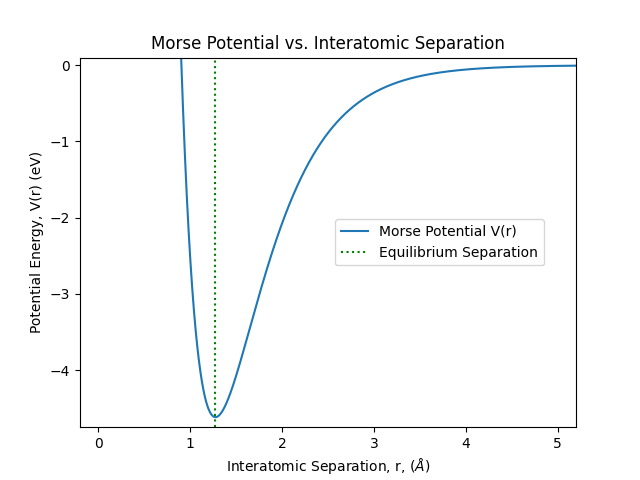
\includegraphics[width=0.67\textwidth]{morse_only.png}
\caption{\label{fig:MorseOnly} Plot of the Morse potential $V(r)$ in eV for the diatomic
molecule HCl versus the interatomic separation $r$ in Å, centered on the region surrounding the
equilibrium separation $r_e$.}
\end{figure}

\section{\label{sec:Results}Results}
Applying the previously described method of finite difference to the diatomic molecule HCl with
parameters shown in Table \ref{tab:MorseVals} yields a calculated ground state energy
$E_0 = -4.434$ eV. This and the next six excited state energy levels are shown in Table
\ref{tab:EnergyLevels} and displayed alongside the Morse potential in Fig.
\ref{fig:MorseLowEnergies} and Fig. \ref{fig:MorseFullSpectrum}, the latter of which includes higher
energy levels closer to the dissociation energy. We then compare the energy levels calculated using finite
difference to those found using the following analytical result:
\begin{align}
    E_n &= h\nu_0(n+1/2) - \frac{[h\nu_0(n+1/2)]^2}{4D_e} \\
    \nu_0 &= \frac{a}{2\pi}\sqrt{\frac{2D_e}{m}} \\
    \implies h\nu_0 &= a\hbar c \sqrt{\frac{2D_e}{mc^2}}
\end{align}
Note that we must subtract the constant energy offset $D_e$ from each analytically calculated
energy level since $E = 0$ is defined as the minimum of the Morse well for the analytical
solution as opposed to the dissociation energy $D_e$ as was defined in this numerical calculation. Here we see
that low energy levels have roughly even spacing, agreeing with that of the traditional quantum harmonic
oscillator. It is only at higher energy level that anharmonic effects have a noticeable perturbation on
the energy level spacing.

\begin{table}
\centering
\caption{\label{tab:EnergyLevels}First seven energy levels for the diatomic molecule HCl calculated
using finite difference and analytical methods.}
\noindent\makebox[\textwidth]{
\begin{tabular}{l|c|c}
Energy Level, $n$ & Numerical Value (eV) & Analytical Value (eV) \\ \hline
$0$ & $-4.43368$ & $-4.43367$ \\
$1$ & $-4.07632$ & $-4.07629$ \\
$2$ & $-3.73399$ & $-3.73393$ \\
$3$ & $-3.40670$ & $-3.40657$ \\
$4$ & $-3.09442$ & $-3.09424$ \\
$5$ & $-2.79717$ & $-2.79692$ \\
$6$ & $-2.51494$ & $-2.51461$
\end{tabular}}
\end{table}

\begin{figure}
\centering
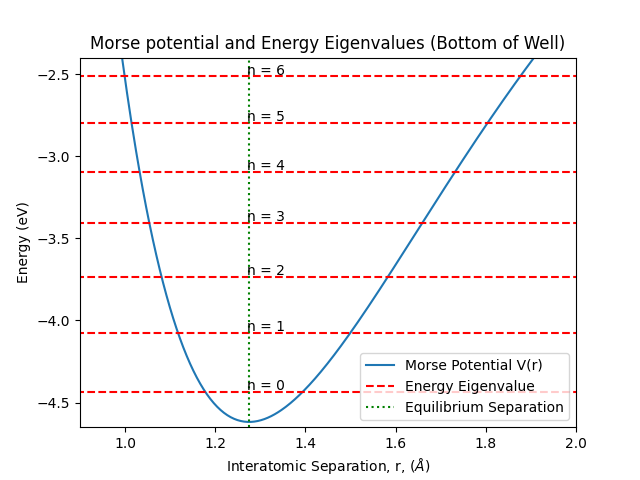
\includegraphics[width=0.67\textwidth]{lower_well_morse_energies.png}
\caption{\label{fig:MorseLowEnergies} Plot of the first seven energy levels alongside the Morse
potential $V(r)$ in eV for the diatomic molecule HCl versus the interatomic separation $r$ in Å
calculated using finite difference.}
\end{figure}

\begin{figure}
\centering
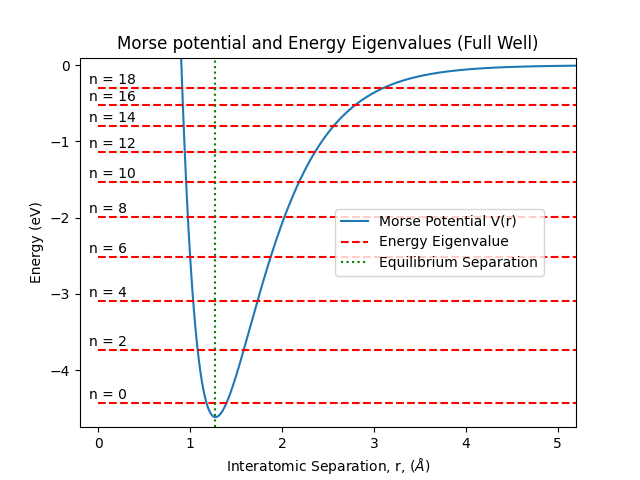
\includegraphics[width=0.67\textwidth]{full_morse_and_energies.png}
\caption{\label{fig:MorseFullSpectrum} Plot of higher energy levels alongside the Morse
potential $V(r)$ in eV for the diatomic molecule HCl versus the interatomic separation $r$. Here we see
anharmonic effects developing at higher energy levels with the separation between adjacent levels decreasing as
$n$ increases.}
\end{figure}

We next extract the eigenstates of this spectral analysis and normalize those of the first three energy
levels for visualization of the corresponding probability distributions, the results of which are shown
in Fig. \ref{fig:MorseProbDistrib}. Here we see similar results to that of the traditional quantum
harmonic oscillator, in which the ground state has interatomic separation close to the equilibrium value
with highest probability. Multiple separations of high probability then develop and shift from the
equilibrium separation as $n$ increases.

\begin{figure}
\centering
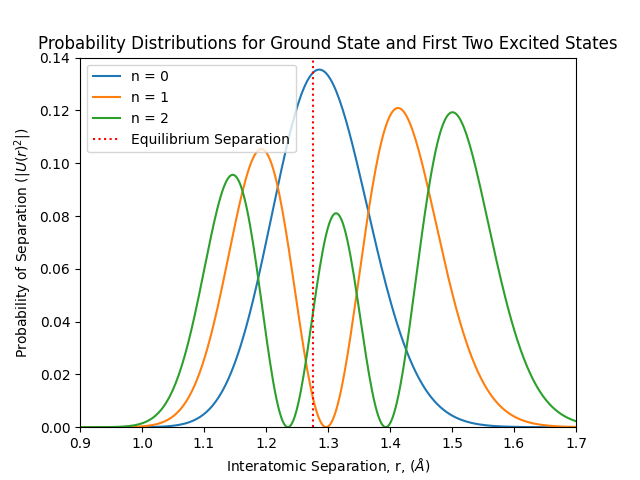
\includegraphics[width=0.67\textwidth]{morse_prob_distribs.png}
\caption{\label{fig:MorseProbDistrib} Plot of probability distributions for the lowest three energy
eigenstates $U_0(r)$, $U_1(r)$, and $U_2(r)$ of HCl in the Morse potential. Here we see modest deviations from the result of the
traditional quantum harmonic oscillator.}
\end{figure}

Finally, we find the interatomic separation probability distribution for the first eigenstate with
calculated energy greater than the dissociation energy $D_e$. We find this to be the $n = 142$ state
with energy $E_{142} = 4.65$ eV (slightly greater than $D_e = 4.618$ eV) and show the corresponding
probability distribution in Fig. \ref{fig:DissocProbDistrib}. Here we see unstable oscillations with
high probability of zero-potential energy separations, indicating that dissociation of the diatomic
molecule can occur.

\begin{figure}
\centering
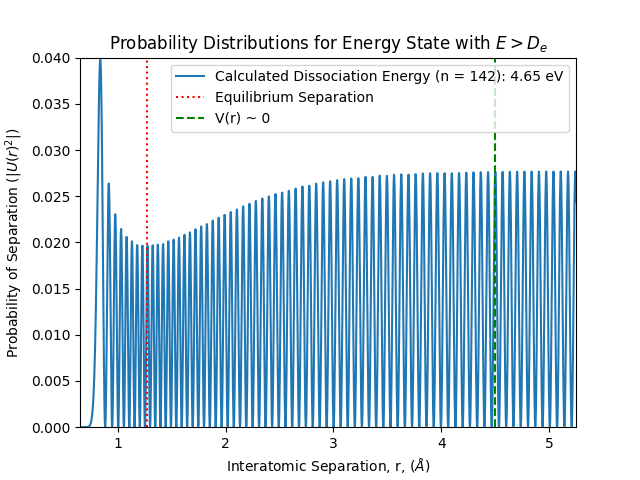
\includegraphics[width=0.67\textwidth]{dissoc_prob_distrib.png}
\caption{\label{fig:DissocProbDistrib} Plot of the probability distribution for the $n = 142$
eigenstate $U_{142}(r)$ of HCl in the Morse potential with energy $E_{142} = 4.65$ eV, just over the
dissociation energy $D_e = 4.618$ eV. The equilibrium separation along with the separation beyond which the
potential energy approaches zero are shown by the dotted red and dashed green lines, respectively.}
\end{figure}

\section{\label{sec:Conclusion_Future_Work}Conclusion and Further Analysis}
We have thus presented a spectral decomposition of the diatomic molecule HCl in a Morse potential
$V(r)$ shown in Eq. \ref{morse2}. We determine the ground state energy of this system to be
$E_0 = -4.434$ eV and display the next six excited state energy levels in Table
\ref{tab:EnergyLevels}. Here we see excellent agreement between the energy levels determined by finite
difference and analytical methods. Fig. \ref{fig:MorseLowEnergies} shows that low energy levels are
roughly equally spaced, agreeing with the result of the traditional quantum harmonic oscillator, while
Fig. \ref{fig:MorseFullSpectrum} shows higher energy states are more closely separated due to
anharmonic effects. This is also shown in Fig. \ref{fig:DissocProbDistrib} by unstable oscillations in
this high-energy wave function leading to dissociation.

Considering future work, one could first optimize the calculation by considering only $r \leq 5$ Å, beyond
which $V(r) \rightarrow 0$. In addition, one could develop a more quantitative comparison between the energy levels of the Morse potential
to those of the traditional quantum harmonic oscillator by numerically calculating successive energy
level differences and comparing to those determined by anharmonicity constants of the HCl system.
Further, one could consider the time evolution of this system using the time evolution operator $U = \exp{(-iHt/\hbar)}$, where H
is the discrete Hamiltonian calculated using finite difference. Finally, it would be interesting to
perform a molecular dynamics simulation by considering the system classically and applying the Verlet
algorithm in which the force acting on each atom is calculated as $F = -dV/dr$ and the atomic positions are
computed by solving Newton's equation. This would allow for the use molecular dynamics software to
visualize molecular motion at low energy states and those near the dissociation energy where bonds can break
from unstable oscillations.

\section{\label{sec:References}References}
\begin{thebibliography}{9}
\bibitem{article}
Srnec MN, Upadhyay S, Madura JD. 2017. A Python Program for Solving Schrodinger's Equation in
Undergraduate Physical Chemistry. J Chem Educ. 94:813-814 

\bibitem{website}
Pulliam T.H. Matrix Form of Finite Difference Schemes. NASA Ames. 2018; [accessed 2022 Feb 6].\\
\href{https://www.nas.nasa.gov/assets/pdf/ams/2018/introtocfd/Intro2CFD_Lecture2_Pulliam_Matrix_ODE.pdf}{https://www.nas.nasa.gov/assets/pdf/ams/2018/introtocfd/Intro2CFD\_Lecture2\_Pulliam\_Matrix\_ODE.pdf}.

\bibitem{presentation}
Fidiani E. Modeling of diatomic molecule using the Morse potential and the Verlet algorithm. AIP
Conference Proceedings 1719, 030001 (2016);
\href{https://doi.org/10.1063/1.4943696}{https://doi.org/10.1063/1.4943696}. Published Online: 11
March 2016.

\bibitem{website}
reduced Planck constant times c in MeV fm. The NIST Reference on Constants, Units, and Uncertainty;
[accessed 2022 Feb 6].
\href{https://physics.nist.gov/cgi-bin/cuu/Value?hbcmevf}{https://physics.nist.gov/cgi-bin/cuu/Value?hbcmevf}.

\bibitem{website}
Conversion from u to eV. The NIST Reference on Constants, Units, and Uncertainty;
[accessed 2022 Feb 6].
\href{https://physics.nist.gov/cgi-bin/cuu/Convert?exp=0&num=1&From=u&To=ev&Action=Convert+value+and+show+factor}{https://physics.nist.gov/cgi-bin/cuu/Convert?exp=0&num=1&From=u&To=ev&Action=Convert+value+and+show+factor}.

\end{thebibliography}

\end{document}
%
% ****** End of file apssamp.tex ******


